\documentclass[12pt]{article}
\usepackage{color}
\usepackage{graphicx}
\usepackage[top=2cm,bottom=2.5cm, inner=1.5cm,outer=1.5cm,twoside,a4paper]{geometry}

\newcommand*{\courierfont}{\fontfamily{pcr}\selectfont}

\begin{document}

\section{Introduction}
Several different tools are used in the GRAND simulation chain~: DANTON down to tau decay, then ZHAireS or RadioMorphing down to electric field computation, and finaly NEC for antenna response computation. Unfortunately, those building blocks do not necessary use the same referential and angular conventions. In this document we detail these conventions and what functions should be called at the interfaces so that conversions are properly handled.

\section{GRAND conventions}  \label{sec:grand}
The GRAND referential (see Fig. \ref{fig:grandref}) is cartesian, defined with x-axis oriented towards the Magnetic North, y-axis towards West and z-axis Up. The GRAND referential is tangential to the Earth surface at sea level at its origin. Obviosuly the GRAND referential can only be a {\it local} one,  with error on angles $>1^{\circ}$ when position is more than 100~km away from the origin. Azimuth angle $\phi$ is measured w.r.t. the x-axis, zenith $\theta$ w.r.t. to z-axis, and in all cases angles are mesured between the direction vectors point to (ie a shower flying South will corespond to $\phi=180^{\circ}$). Consequently a shower flying downward will correspond to $\theta>90^{\circ}$, which is opposite to the usual cosmic-ray convention. 
%
\begin{figure}[ht]
\centering
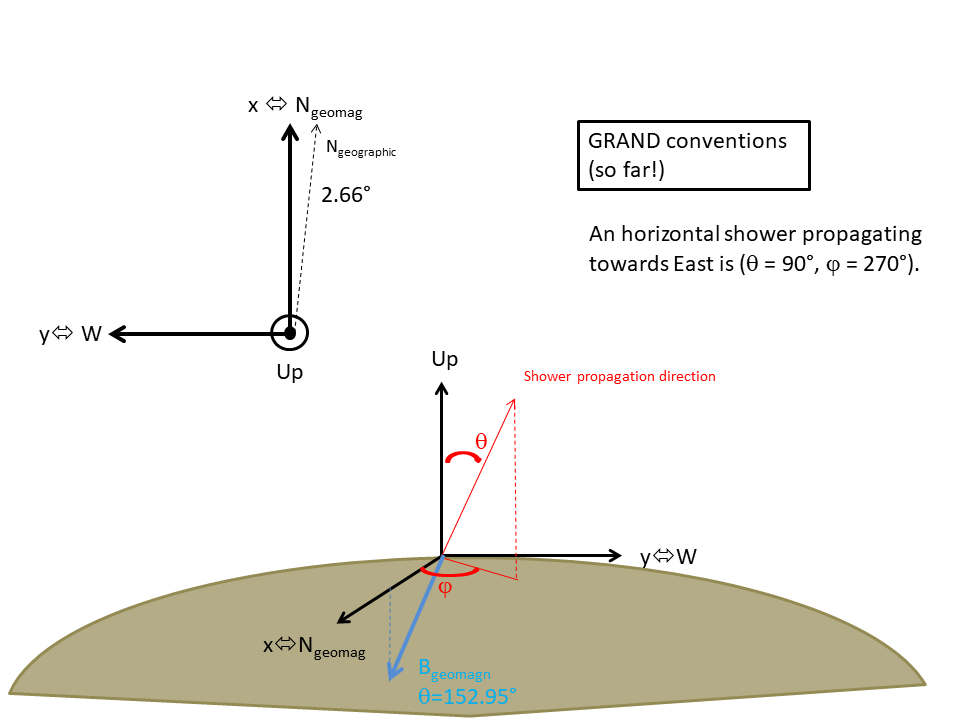
\includegraphics[width=\textwidth]{GRANDreferential.png} 
\caption{\label{fig:grandref} Sketch showing the GRAND coordinate system. The arrow is pointing towards the direction where the air showers goes to. This means a shower with a zenith of $\theta_mathrm{GRAND}<90^\circ$ is up-going.}
\end{figure} 

\section{DANTON}  \label{sec:danton}
{\bf To be completed: general idea, input...}
%
\subsection{Output file format}
DANTON output files are tables in text format which include informations on the momentum of the tau decay daughter particles in the columns ($p_x$, $p_y$, $p_z$) (in units of GeV/c), where the x-axis is the projection of the shower unitary vector along the horizontal direction and the z-axis its projection along the vertical.  \\
The function {\bf xxx} in script {\bf yyy}\footnote{This script, as all other mentionned in this note, is stored in https://github.com/grand-mother/simulations.} allows computing the zenith and azimuth angles corresponding to the momentum vector ($p_x$, $p_y$, $p_z$), using GRAND conventions.

%
\section{ZHAireS}\label{sec:zhaires}
The AIRES referential is identical to GRAND: x-axis oriented towards the Magnetic North, y-axis towards West and z-axis Up. However, following the standard cosmic-ray conventions, the angles are mesured w.r.t the direction where the air shower comes from, opposite to GRAND (see section \ref{sec:grand}). This leads to following conversion:
\[\phi_{GRAND}=180^\circ +\phi_{Aires}\] and \[\theta_{GRAND}=180^\circ -\theta_{Aires} \]
However in ZHAireS, the radio extension of AIRES, the z-axis is reverted compared to AIRES and points down, with an origin set at 100~km above the Earth surface. Therefore positions and z-componant of vectors have to be reverted when switching back to GRAND conventions~:\\
    \[E_z(t)=-1 \times E_{z,sim}(t) \] and
    \[z_{GRAND}= 100,000\,\mbox{m}-z_{ZHAIreS} \]
This applies in particular to the antenna positions and the electric field vector read in the {\courierfont time-fresnel.out} output file of ZHAireS simulations.
{\bf Add something about ZHAireS inputs and scripts to call them.}

\section{NEC}\label{sec:nec}
The antenna response to radio waves is computed in the {\courierfont get\_voltage()} function of the {\courierfont computevoltage.py} script. Azimuth and zenith angle are handed to {\courierfont get\_voltage()} in GRAND conventions but are internaly converted in NEC conventions, where x-axis point towards East, y-axis towards North and z-axis points Up. Azimuth angle $\phi$ is measured w.r.t. the x-axis, zenith $\theta$ w.r.t. to z-axis but using cosmic-ray conventions ($\theta<90^{\circ}$ for a shower flying downward). Consequently following conversions formulas are applied between GRAND and NEC referentials~:
\[\phi_{response}=\phi_{GRAND}+90^\circ\] an
\[\theta_{response}= 180^\circ-\theta_{GRAND}\] 
These formulas are directly implemented in the {\courierfont GRANDtoNEC()} function in {\courierfont computevoltage.py}.
Note also that inside {\courierfont get\_voltage()} a {\it local referential} ($\vec{e_r},\vec{e_\phi},\vec{e_\theta}$) is used, where $\vec{e_r}$ is a radial vector parallel to the wave propagation axis and pointing to the antenna, and ($\vec{e_\phi},\vec{e_\theta}$) define the E-field plane with $\vec{e_\phi}$ such as $\vec{e_\phi}\cdot\vec{e_z}=0$.
Following forumals are therefore used to compute the E-field componants in the ($\vec{e_r},\vec{e_\phi},\vec{e_\theta}$) referential~: \\
\[E_r(t)=0 \] (following the plane wave approcimation)
\[E_\theta = \cos\theta_{NEC}(\cos\phi_{NEC} E_{yGRAND} - \sin\phi_{NEC}E_{xGRAND})-\sin\theta_{NEC}E_{zGRAND} \] 
\[E_\phi = -\sin\phi_{NEC}E_{yGRAND}-\cos\phi_{NEC}E_{xGRAND} \]

\end{document}
